\documentclass[11pt]{article}
\usepackage[hmargin=1in,vmargin=1in]{geometry}
\usepackage{xcolor}
\usepackage{amsmath,amssymb,amsfonts,url,sectsty,framed,tcolorbox,framed,graphicx}
\newcommand{\pf}{{\bf Proof: }}
\newtheorem{theorem}{Theorem}
\newtheorem{lemma}{Lemma}
\newtheorem{proposition}{Proposition}
\newtheorem{definition}{Definition}
\newtheorem{remark}{Remark}
\newcommand{\qed}{\hfill \rule{2mm}{2mm}}


\begin{document}
\noindent
\rule{\textwidth}{1pt}
\begin{center}
{\bf [CS304] Introduction to Cryptography and Network Security}
\end{center}
Course Instructor: Dr. Dibyendu Roy \hfill Winter 2022-2023\\
Scribed by: Srushti Rathva (202051183) \hfill Lecture (Week 2)
\\
\rule{\textwidth}{1pt}

\section*{Hill Cipher}
It encrypts groups of letters at a time, rather than individual letters. The size of the block is determined by the size of the key matrix. \\
$ A \rightarrow $ Secret key \\
$ M \rightarrow $ Plaintext \\
$ C \rightarrow $ Ciphertext \\
$ M = m_1 m_2 ... m_n $ \\
\textbf{Note} : A should be \textbf{invertible matrix}.
\\ \\
\textbf{Encryption} \\
C = A*M = $ (c_1 c_2 ... c_n) $ 
\\ \\ 
\textbf{Decryption} \\
M = $ A^{-1} $*C = $ (m_1 m_2 ... m_n) $ 

\section*{Kerckhoff's Rule}
Design of the cryptographic algorithm should be public.\\
In other words, the security of the system should not rely on the secrecy of the algorithm or the method of encryption, but rather on the secrecy of the key. 

\section*{Shannon's notion of perfect secrecy}
$ E \rightarrow $ Encyption key \\
$ P \rightarrow $ Plaintext \\
$ C \rightarrow $ Ciphertext \\
then, E(P) = C \\ \\
E will provide perfect secrecy iff the ciphertext does not reveal any information about plaintext. \\ \\
It refers to a system of encryption where the ciphertext provides no information about the plaintext, regardless of the amount of ciphertext or any prior knowledge a person may have about the plaintext or the encryption method. \\ \\
$ P_r = 
\begin{bmatrix}
    M = m & | & C = c \\
\end{bmatrix} 
= 
\begin{bmatrix}
    M = m \\
\end{bmatrix} 
\\ \\
P_r = 
\begin{bmatrix}
    Message & | & Ciphertext \\
\end{bmatrix} 
= 
\begin{bmatrix}
    Message \\
\end{bmatrix} 
$
\section*{Symmetric Key Cipher}
\begin{center}
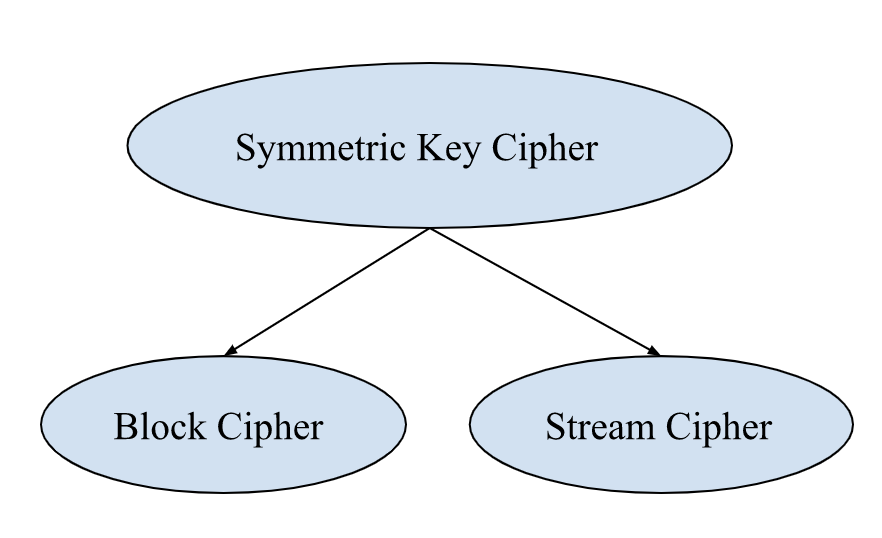
\includegraphics[width=250pt]{p1.png}
\end{center}

\subsection*{Block Cipher}
Message is divided into blocks of fixed size and then each block is encrypted separately. \\ 
$
M = m_0 || m_1 || ... || m_n \\
len(m_i) = l \\ 
C = E(m_0,k) || E(m_1,k) || ... || E(m_n,k) = C = c_0 || c_1 || ... || c_n 
$

\subsection*{Stream Cipher}
Encryption is done bit wise. \\ 
$
M = m_0m_1...m_n \\
m_i \in {0,1} \\ 
C = (m_0 \oplus z_0,m_1 \oplus z_1, ... m_i \oplus z_i) \\
M = (c_0 \oplus z_0,c_1 \oplus z_1, ... c_i \oplus z_i)  \\
$

\section*{Product Cipher}
It combines two or more simpler cryptographic primitives (such as substitution and transposition) in order to achieve a higher level of security. 

\subsection*{Substitution Permutation Network}
It is a product cipher based on substitution box and permutation box.\\
$
S : \{0,1\} ^n \rightarrow \{0,1\} ^m \\
P : \{0,... mr-1\} \rightarrow \{0,... mr-1\}
$
\begin{center}
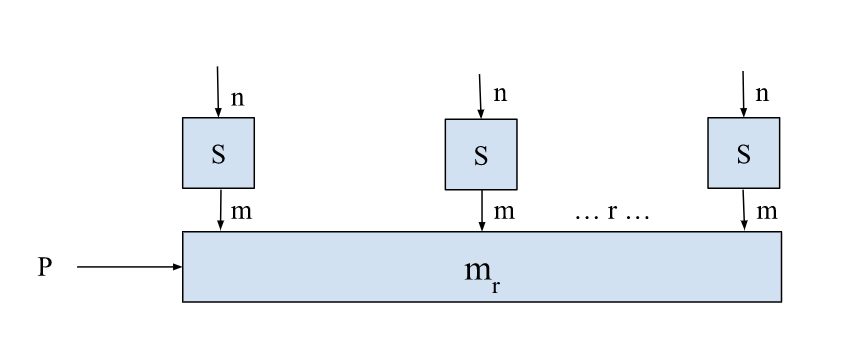
\includegraphics[width=250pt]{p2.png}
\end{center}

\subsection*{Feistel Network}
P $ \rightarrow $ Plaintext of size 2n \\
P = $L_0 || R_0$ \\
K $ \rightarrow $ Secret key \\
len(K) = $l$ bits \\
$ f : \{0,1\}^n X \{0,1\}^l \rightarrow \{0,1\}^n $
\\ \\
\textbf{Encryption} \\
$
L_1 = R_0 \\
R_1 = L_0 \oplus f(R_0,K) \\
C = L_1 || R_1 \\
$
\begin{center}
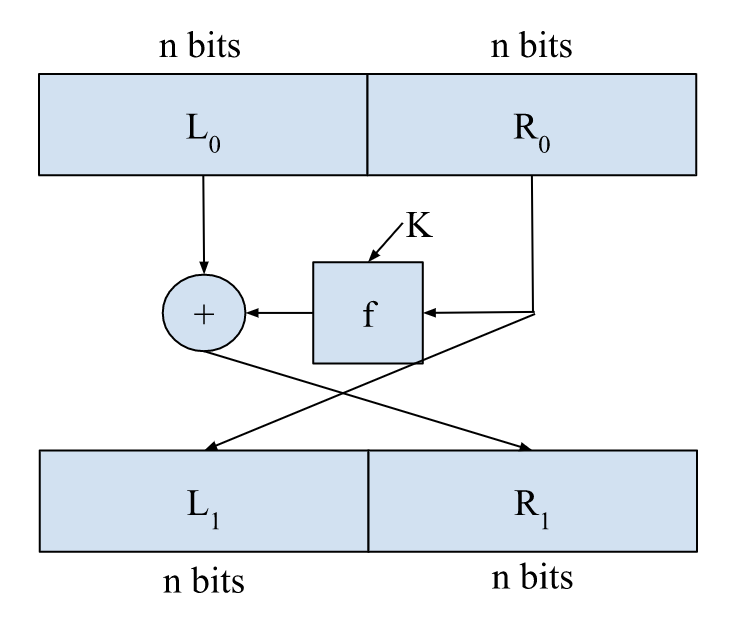
\includegraphics[width=200pt]{p3.png}
\end{center}
\textbf{Decryption} \\
$
R_0 = L_1 \\
L_0 = R_1 \oplus f(L_1,K) \\
P = L_0 || R_0 \\
$
\begin{center}
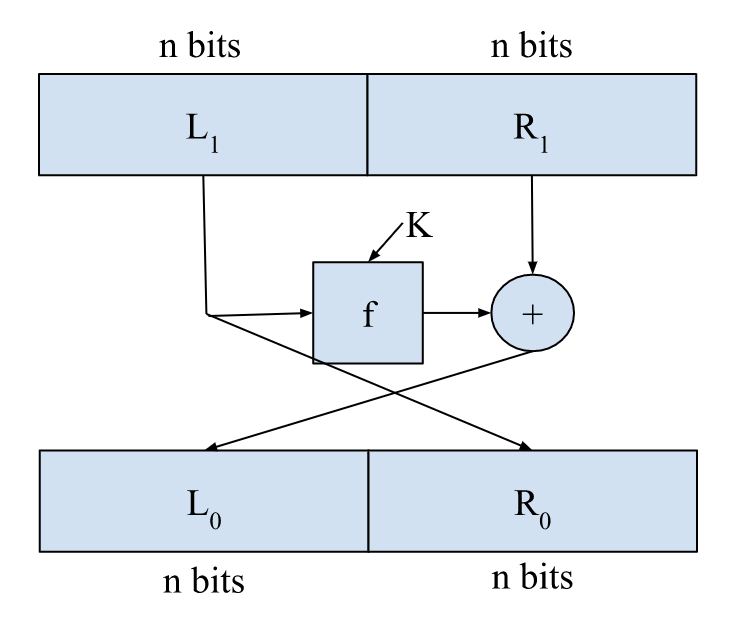
\includegraphics[width=200pt]{p4.png}
\end{center}

\subsection*{Iterated Block Cipher}
It is a block cipher involving the sequential repetition of an internal function called as round function. \\
Parameters : \\
$ r \rightarrow$ Number of rounds \\
$ n \rightarrow$ Block size \\
$ k_i \rightarrow$ Generated round keys of length $l$ from original secret key $K$\\
$G(K) \rightarrow k_1 , k_2 , k_3 \rightarrow$ round keys \\
$F \rightarrow$ round function \\
\begin{center}
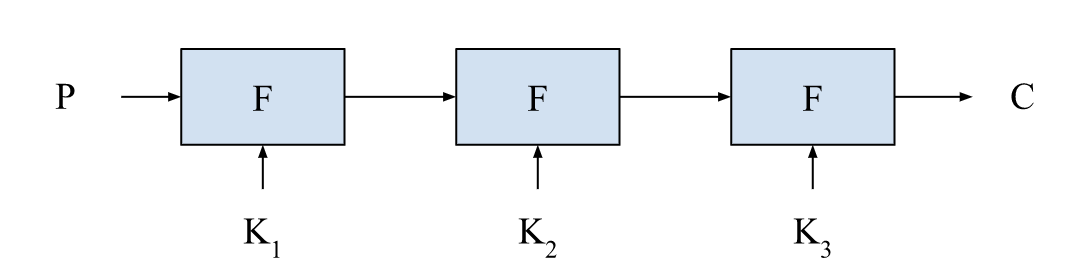
\includegraphics[width=250pt]{p5.png}
\end{center}

\section*{One Time Padding (OTP)}
OTP provides perfect secrecy under some conditions. \\ \\
\textbf{Encryption} \\
$ P \rightarrow$ Plaintext \\
$ K \rightarrow$ Secret Key \\
$ E(P,K) \rightarrow P \oplus K = C$ \\ \\
\textbf{Decryption} \\
$ C \rightarrow$ Ciphertext \\
$ K \rightarrow$ Secret Key \\
$ D(C,K) \rightarrow C \oplus K = P$ \\ \\
\textbf{Conditions}\\
1. The secret key $K$ can not be used to encrypt two messages \\
2. length($K$) $\geq$ length($P$) \\
3. $K$ is uniformly selected from the key space \\
\end{document}